
\section{Interference of Light From Two or More Slits}
\label{interference_lab}
\makelabheader %(Space for student name, etc., defined in master.tex)

\instructornote{%
Major rewrites by Matt in 2015, 2019.  Time: long, if you do all of it.

(Based on earlier version that was worked on by Jerry et al.) 

As of 2019, this lab now integrated with the use of a Mathematica notebook to help students visualize what's happening.

This lab is designed to be a standalone introduction to two-slit interference, with no need for any introductory lecture.  Alternatively, since the activities are designed to be somewhat independent of each other, you could imagine covering the derivation in a lecture and skipping activity 3 (though that would miss the Mathematica visualization).  Activity 5, which is about more than two slits, could also be completely skipped if you're pressed for time.
}

\medskip
\textbf{Objective}

In this laboratory you will investigate the wave-like nature of light by measuring the interference 
between light beams produced by a laser shining through a set of narrow, adjacent
slits. 
%\begin{itemize}
%\item To investigate the interference of light waves as they pass through
%a set of slits. 
%\end{itemize}

\medskip
\textbf{Apparatus}

\begin{itemize}[nosep]
\item Basic optics diode laser
\item Optical bench with rotary motion sensor
\item Phototransistor for measuring light intensity (mounted on rotary motion sensor)
\item ``Multiple Slit Set'' slit accessory
%\item ``Single Slit Set'' slit accessory
\item Small plastic ruler
%\item Glass plate with sets of narrow slits
\item Pasco 550 Interface 
\item \textit{Capstone} software (\filename{Interference.cap} experiment file)
\item \textit{Mathematica} software (\filename{interference.nb} notebook file)
\end{itemize}


\medskip
\textbf{Activity 1: An Alternative View of Light}

Isaac Newton believed that light was made up of small, unseen particles, or ``corpuscles,''
that obeyed (surprisingly enough!) Newton's Laws. 

%This view is known
%as the corpuscular theory. Let's briefly consider how this model of light
%predicts different behavior from the wave theory.

(a) Consider a laser beam shining on a circular hole. If a beam of
light consisted of small, unseen particles that behaved as tiny billiard
balls, what would you see on a screen that is downstream from the circular
hole?  (This question and the next one aren't meant to be hard.
They're just getting at your common sense notions about how shadows work.)

%\begin{center}
{\centering 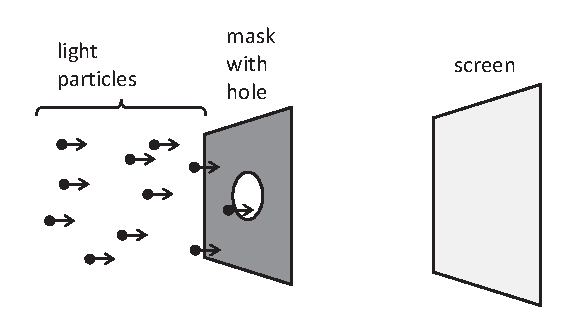
\includegraphics[scale=0.85]{interference_of_light/circular_hole.eps} \par}

%\end{center}

(b) Now consider the same laser beam shining on a pair of narrow slits.
What would you see on a screen downstream from the slits if light
were made of corpuscles?

%\begin{center}
{\centering 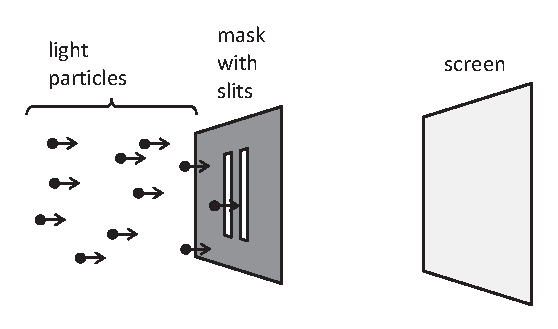
\includegraphics[scale=0.85]{interference_of_light/particles_two_slits.eps} \par}
%\end{center}

You probably predicted that the laser would
form a single bright spot for part (a) and two parallel bright lines for part
(b).  In fact, the experiment you are about to perform challenges Newton's corpuscular theory. 
You'll see something very different for light shining through two narrow slits.

%\bigskip

\textbf{Activity 2: Experimental Setup for Measuring the Interference of Light (and First Data)}

You will measure this ``interference pattern'' with the setup shown below. 
(This is a \textit{top} view of the set-up.) 
The detector assembly includes a light sensor mounted on a rail. The sensor converts the intensity 
of the light that hits it into a voltage signal that can be read by the
computer. In addition, the sensor can be moved back and
forth on a rotary motion sensor that measures the sensor's position. These two signals can be combined to
make a graph of the intensity as a function of position.

%\answerspace{0.3cm}
%{\centering \resizebox*{0.75\textwidth}{!}{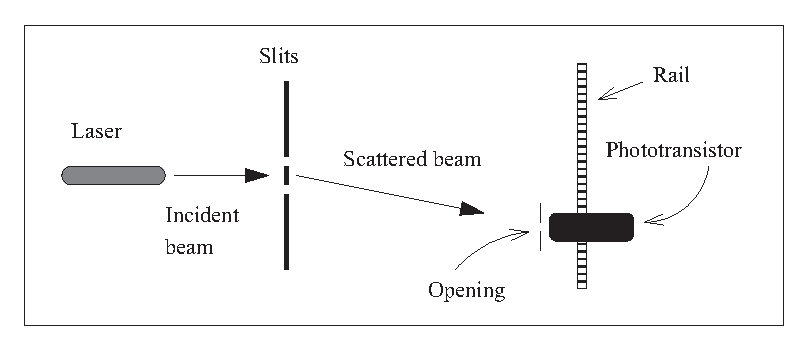
\includegraphics{interference_of_light/interference_of_light_fig1b_bw.eps}}
%\begin{center}
{\centering 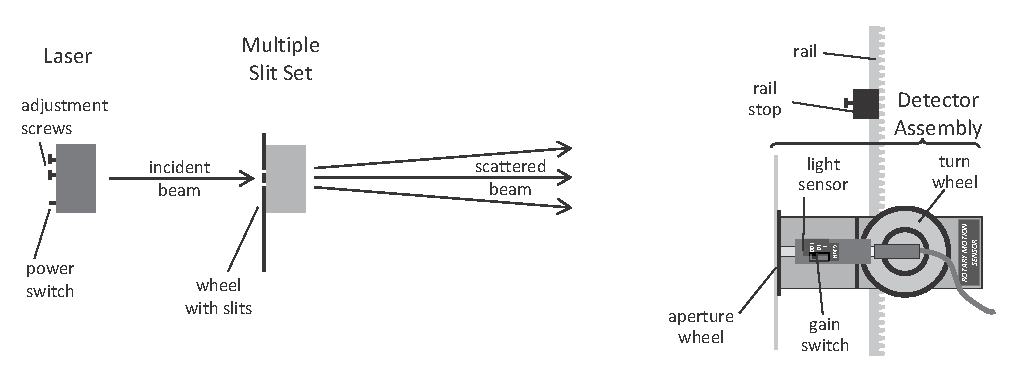
\includegraphics[width=0.95\textwidth]{interference_of_light/apparatus.eps} \par}
%\end{center}
\label{figure_rail_stop}
%\answerspace{0.3cm}

(a) Mount the laser on the 
optical bench at the opposite end from the detector assembly.
DO NOT LOOK DIRECTLY INTO
THE BEAM.  Turn on the
laser.  You should see the bright red spot of the beam striking
the aperture wheel and the small white screen in front of the light sensor. 
Use the two adjustment screws on the back of the laser to to make the beam hit the exact center of the opening in front of the light sensor (the ``aperture'') when it is positioned in the middle of its travel range.  

%\vspace{10mm}

(b) Identify the ``Multiple Slit Set'' slit accessory.  You will place this on the optical bench near the laser, about 70 or 80 cm away from the detector assembly.  Select a double slit of width .04 mm and separation .125 mm, marked by the number ``2''. You can rotate the wheel with the slits AND rotate where the slit wheel is mounted on the plastic frame.  
Rotate both so that when you click the frame onto the optical bench, the double slit that you want is at the center of the opening, with the slits oriented vertically and the laser beam centered right on it.  You should now see the ``interference pattern,'' consisting of a series of bright spots a few millimeters apart, on the white screen in front of the light sensor.

%\vspace{10mm}

(c) On the light sensor itself, set the small gain switch to ``100'' (highest sensitivity).  Rotate the aperture wheel in front of the sensor to the position marked ``3''.  (Wider gaps let in more light; narrower gaps measure light at a more precisely defined location.)  Also check that the sensor is exactly perpendicular to the incident beam; adjust its mounting if necessary.

%\vspace{10mm}

(d) Open the file \filename{Interference.cap} in the \filename{\coursefolder} folder. 
When you are ready, click \button{Record} and slowly move the detector assembly 
from one side of the bright spots to the other by rotating the positioning wheel on the rotary 
motion sensor. Move carefully and take about ten seconds to complete the 
motion. 
As you move it, the computer screen should show a graph of the intensity reading versus the position reading. 
Click \button{Stop} when you're done. 
The graph, called the interference pattern, should be a symmetric pattern of distinct peaks. Consult your instructor if your setup isn't working.

%\pagebreak[2]
(e) In the space below, draw a good graph showing your interference pattern.  
Be sure to label your axes!
\textit{(If your instructor requests it, make a hardcopy of this graph and attach it to this unit.)}

\answerspace{1.0in}


\pagebreak[2]
\textbf{Activity 3: Understanding What's Going On, and Deriving Locations of Bright Spots}

%Let's think about why your interference pattern looks the way it does.  
When the laser hits the two slits, 
light comes out of the slits in all directions all at once, as in the diagram (a) below.  
But that's a lot of light rays to keep track of, so we'll focus on just two at a time, always in the same direction, as in (b) below.
We'll define $\theta$ as the angle of the rays, where $\theta=0$ means straight ahead.  

{\centering 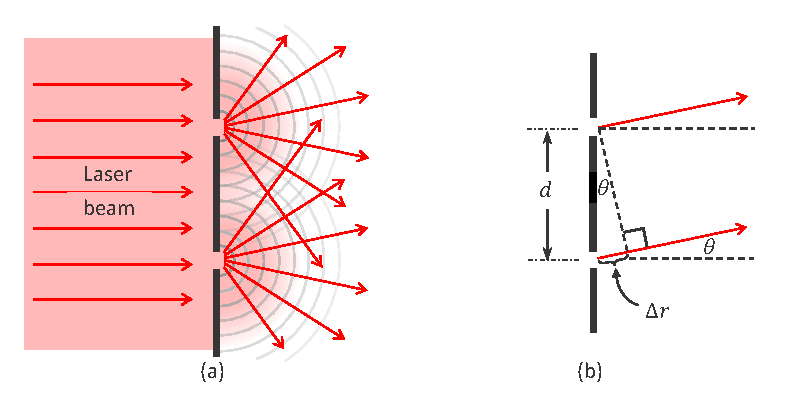
\includegraphics[width=0.63\textwidth]{interference_of_light/rays2_color.eps} \par}
\index{color page}

The pair of rays are aimed at the same spot on the screen or at the detector, 
but they travel slightly different distances to get there.  
The difference in path length, shown on the diagram as $\Delta r$, leads to \textit{interference} between the two rays, which causes the 
bright and dark areas you see on the screen.

To help you visualize what's happening, open the file \filename{interference.nb} in the \filename{\coursefolder} folder; 
it will open in \textit{Mathematica}.  Hit \button{Control-A} to select all the text, and \button{Shift-Enter} 
to execute all of the selected text.  Scroll down until you see the graphics, and make the window full screen so the graphics all fits side by side.  You should see something like the screen shot below.

%{\centering \includegraphics[height=4.1in]{interference_of_light/simulation_screenshot.eps} \par}
{\centering 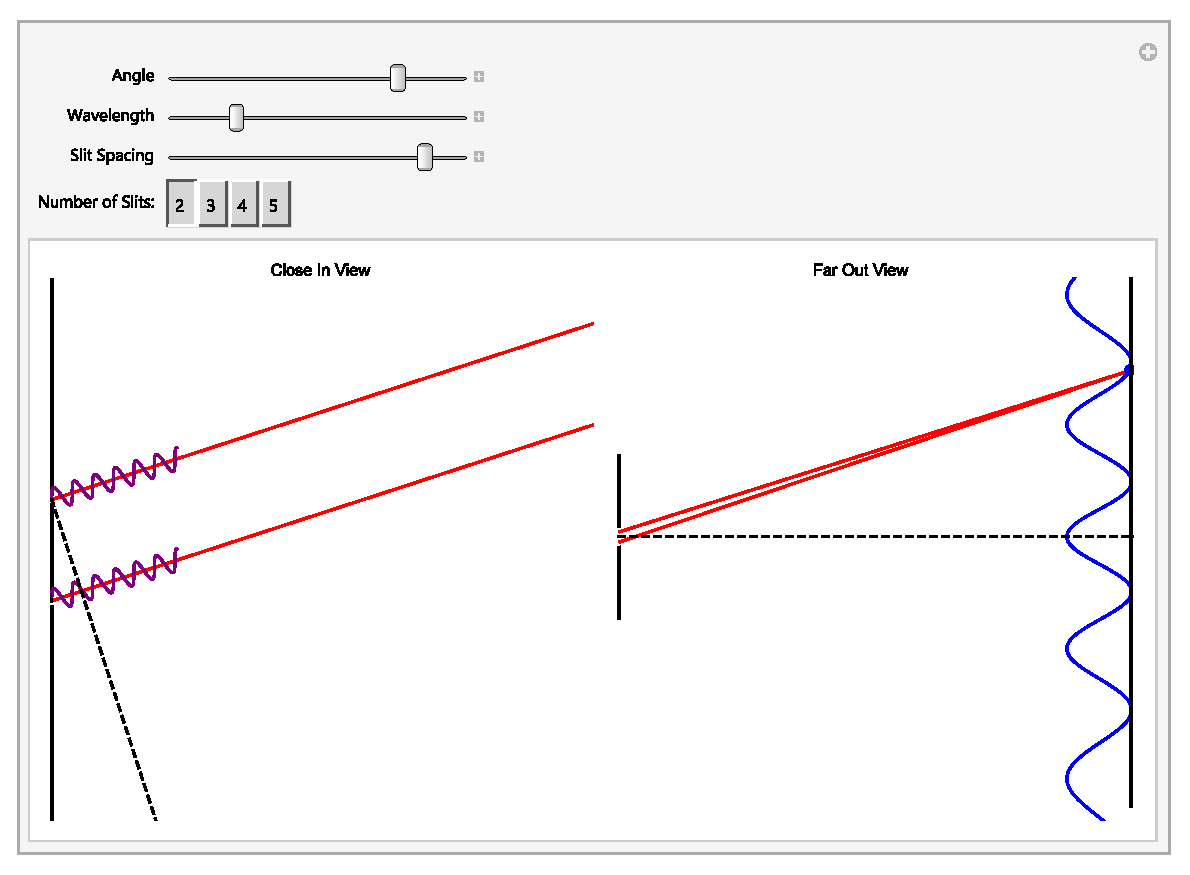
\includegraphics[height=4.1in]{interference_of_light/screengrab.eps} \par}
\index{color page}

One little detail: You might ask, ``Wait!  How can the two rays converge at the detector if they're parallel?!?''  The answer is that they're not \textit{perfectly} parallel, but they're pretty close, as the ``Far Out View'' in the simulation above suggests.  In your experimental setup, the two slits are only separated by a fraction of a millimeter, and the detector is almost a meter away.  The math is way easier if we approximate the rays as parallel.


\pagebreak[2]
(a) For a particular angle $\theta$, if the path difference $\Delta r$ happens to be an exact integer multiple of the light's wavelength $\lambda$, will the two waves combine \textit{CON-structively} or \textit{DE-structively}?  And does that correspond to a bright spot or a dark spot?  (To see this in the simulation, drag the \button{Angle} slider so that the diagonal dashed line in the left figure crosses the lower ray at exactly one wavelength from the lower slit.  The blue graph on the far right will show the resulting light intensity at that angle.)
\answerspace{0.5in}

(b) For a particular angle $\theta$, if the path difference $\Delta r$ happens to be an exact half-integer multiple of the light's wavelength $\lambda$ (like $0.5\lambda$ or $3.5\lambda$), will the two waves combine \textit{CON-structively} or \textit{DE-structively}?
\answerspace{0.5in}

(c) What about if the path difference $\Delta r$ happens to be something in between, like $\Delta r = 2.3\lambda$, or $0.75\lambda$? Would that place on the screen be maximally bright? Or totally dark? Or something in between?
\answerspace{0.5in}

\textit{Now you have the basic idea: As $\theta$ increases from $0^\circ$,
% at the center, 
the path difference $\Delta r$ increases, and the interference between the two rays alternates between constructive and destructive, causing the oscillating interference pattern you measured.}


(d) On your graph, the highest maximum is straight ahead of the slits ($\theta=0^\circ$), where $\Delta r=0$.  Now consider rays at an angle $\theta$ leading to the \textit{next} maximum, just to the right of the center.  At that angle $\theta$, what is $\Delta r$ in terms of $\lambda$?   ($\Delta r=\frac{1}{2}\lambda$?  Or $\Delta r = \lambda$?  Or $2\lambda$?) 

\vspace{0.1in}
\hspace{0.8in}$\Delta r=$
\vspace{0.1in}

(e) Are the two $\theta$'s in (b) of the drawing on the last page the same?
\answerspace{0.2in}

(f) Write $\Delta r$ in terms of the distance between the slits $d$ and the the angle $\theta$.
\answerspace{0.4in}

(g) At angles for which $d \sin \theta = 0$, is the intensity a maximum or a minimum?
\answerspace{0.2in}

(h) At angles for which $d \sin \theta = \lambda$, is the intensity a maximum or a minimum?
\answerspace{0.2in}

(i) At angles for which $d \sin \theta = 2 \lambda$, is the intensity a maximum or a minimum?  What about $d \sin \theta = 37 \lambda$?
\answerspace{0.2in}

Congratulations!  You've just derived that the intensity maxima in your measured interference pattern should occur wherever $\Delta r$ is any integer multiple of $\lambda$, so in general there are intensity maxima at any $\theta$ where
\begin{equation}
d \sin \theta = m \lambda,
\end{equation}
where $m$ is some integer 0, 1, 2, 3, and so on.  



\pagebreak[3]
\textbf{Activity 4: Determining the Wavelength of the Laser }

Now you'll use the geometry of your setup to measure the actual wavelength $\lambda$ of the light from your laser!




(a) Write $\theta$ in terms of the length $L$ between the detector and the slits and the horizontal distance $\Delta x$ between the central maximum and the next maximum to the right of it.
\answerspace{0.4in}

(b) Measure $L$ carefully.  (The part inside the light sensor that actually \textit{does} the sensing is located 25 mm behind the plane of the aperture wheel.)  
Also measure $\Delta x$.  (Hint: if you use the \button{Coordinates/Delta Tool} to read exact values, you will need to increase the number of significant digits shown; see Appendix \ref{capstone}.)
Record your values for $L$, $\Delta x$, and $\theta$ here.

\answerspace{0.8in}

(c) In equation (1) on the previous page, what value of $m$ corresponds to the maximum right next to the central maximum in your interference pattern?
\answerspace{0.3in}
 
(d) Look back at part (b) of Activity 2 to recall the distance $d$ between the two slits, and write it below.
\answerspace{0.3in}

(e) Combine your answers for parts (b) through (d) to calculate a value for $\lambda$.  
\answerspace{1in}

(f) Does your value correspond to an accepted value for red light?
\answerspace{0.3in}

(g) Try calculating the wavelength of the laser light again, this time using the distance between the central maximum ($m=0$) and the maximum for $m=3$.  (If $m=3$ is hard to see, $m=2$ is okay too.)
\answerspace{0.9in}


\pagebreak[2]
\textbf{Activity 5: More Than Two Slits}

(a) What if, instead of two slits, you shined the laser on a series of three or four slits, all equally spaced?  Would you still see an interference pattern?  Would the spacing between maxima be the same?  What is your prediction?
\answerspace{0.8in}

(b) To look for any differences, you will want to have the smoothest, nicest interference pattern you can get.  Take data for the two-slit interference pattern again to get it \textit{really} pretty.  Also, this time start with the detector assembly butting up against the rail stop (see the diagram on page \pageref{figure_rail_stop}), so that you can start from the exact same location each time.

(c) Now, without deleting your previous data, switch to three slits by rotating the wheel on the slit accessory 
to ``3'', and record the interference pattern produced.
To make your two graphs align, start with the detector assembly butting up against the rail stop as before.  
What about the interference pattern has changed, and what has stayed the same?
\answerspace{0.8in}

(d) What happens with four slits?  Or five slits?
\answerspace{0.8in}

(e) Suppose we have three slits all a distance $d$ apart, and we draw three parallel rays from them, 1, 2, and 3.  For an angle $\theta$ at which the path difference between rays 1 and 2 just happens to be $\Delta r_{12} = \lambda$, what is the path difference $\Delta r_{13}$ between rays 1 and 3?  (To check yourself, you can look again at the simulation, changing the number of slits by clicking on \button{3}.

%\answerspace{1.5in}
\hspace{0.5in}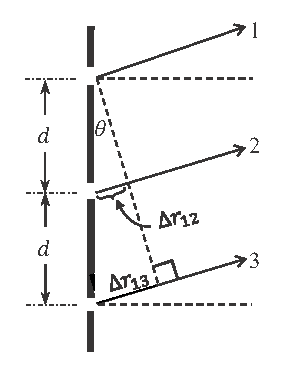
\includegraphics[width=1.7in]{interference_of_light/three_slits.eps}

(f) Is there any angle $\theta$ at which rays 1 and 2 interfere perfectly constructively with each other,  but ray 3 interferes destructively with either of them?
\answerspace{0.3in}

\textit{Okay then: It seems that the brightness maxima for LOTS of slits are at the same places as for just two slits.}

\pagebreak[2]
(g) Suppose you have four rays, 1, 2, 3, and 4, and suppose we consider an angle $\theta$ at which the path difference between the first two is $\Delta r_{12} = 0.75\lambda$ as shown below.  What are the distances $\Delta r_{13}$ and $\Delta r_{14}$?

%\answerspace{2.5in}
\hspace{0.5in}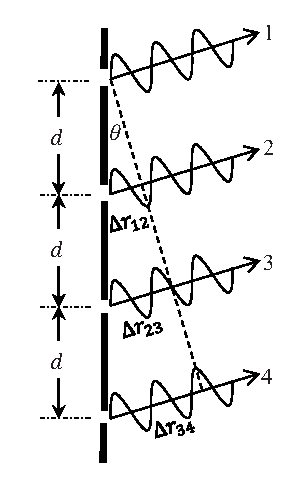
\includegraphics[width=1.5in]{interference_of_light/four_slits.eps}

(h) In the case in (g), would rays 1 and 3 interfere \textit{CON-structively} or \textit{DE-structively}?  How about rays 2 and 4?
\answerspace{0.5in}

(i) If you combined all four rays together, would the result at the detector be a place of high intensity or low intensity? 
\answerspace{0.3in}

(j) Check your answer in part (i) by setting up the situation pictured above in the simulation using four slits.  Were you correct?
\answerspace{0.2in}


(k) If there were only TWO slits, and you combined only TWO rays together with a path difference of $\Delta r_{12} = 0.75\lambda$, would the result at the detector be a place of high intensity or low intensity, or something in between? 
\answerspace{0.4in}

\textit{Okay then: So at a $\theta$ just a LITTLE bit off from a maximum, with two slits you still have mostly constructive interference.  But with lots of slits you have way more opportunities for DE-structive interference.}

(l) In general, as you increase the number of slits, does the maximum brightness of the intensity maxima increase or decrease? Does the width of the intensity maxima increase or decrease?

%\answerspace{0.6in}

\medskip
\hspace{0.5in} More slits $\Longrightarrow$ Brightness:
\medskip

\hspace{0.5in} More slits $\Longrightarrow$ Width:
\medskip


\textbf{Activity 6: One More Thing...}

Remember the earlier discussion in Activity 1 of Newton's corpuscular theory of
light? You've taken a ton of data by now.  Which theory does your data support: Newton's corpuscular theory of light or the wave theory of light?
Explain.
\answerspace{\fill}
